\documentclass[journal]{IEEEtran}

\usepackage{amsmath, amssymb}
\usepackage{graphicx}
\usepackage{hyperref}
\usepackage{cite}
\usepackage{booktabs}
\usepackage{color}
\usepackage{tikz}
\usepackage{pgfplots}
\pgfplotsset{compat=1.17}

\begin{document}

% \title{Ising Clustering: A Democratic Voting Approach}

\title{
Ising Clustering: A Democratic Voting Approach\\
%\thanks{
%This work is supported in part by the Research Grants Council (GRF 17201822 and TRS T45-701/22-R) of Hong Kong SAR, China; and in part by the Department of Science and Technology of Guangdong Province (2023B0909020003).}
}

\author{\IEEEauthorblockN{Rongzhou Chen\textsuperscript{1}, Yuqing Cao\textsuperscript{1}, 
% Yaping Zhao\textsuperscript{1}, 
Mengfan Liu\textsuperscript{2}, Chuan Wu\textsuperscript{2,$\dag$}, Edmund Y. Lam\textsuperscript{1,*}}\\
\IEEEauthorblockA{\textit{\textsuperscript{1}Department of Electrical and Electronic Engineering, The University of Hong Kong, Hong Kong SAR of China} \\
\textit{\textsuperscript{2}Department of Computer Science, The University of Hong Kong, Hong Kong SAR of China}
\\
\texttt{\textsuperscript{*}elam@eee.hku.hk} \ \texttt{\textsuperscript{$\dag$}cwu@cs.hku.hk}}
}


\maketitle

\begin{abstract}
Clustering is a fundamental task in unsupervised learning, aiming to group similar data points without prior labels. Traditional clustering methods often struggle with complex data structures and require careful parameter tuning. In this paper, we introduce \textit{Ising Clustering}, a novel algorithm inspired by the Ising model from statistical physics. We provide a mathematical derivation to demonstrate that Ising Clustering can be formulated as an optimization problem, which can be further reformulated to the Quadratic Unconstrained Binary Optimization (QUBO). By employing a neural network with a softmax output layer and maximizing pairwise differences among samples, our method implements a democratic voting mechanism that promotes well-separated clusters. We validate the effectiveness of our proposed algorithm through experiments on benchmark datasets.
\end{abstract}

\begin{IEEEkeywords}
Clustering, Ising Model, Neural Networks, Unsupervised Learning, Pairwise Difference Loss, QUBO.
\end{IEEEkeywords}

\section{Introduction}

\IEEEPARstart{C}{lustering} is an essential technique in exploratory data analysis, with applications ranging from image segmentation to bioinformatics~\cite{jain1999data}. Classical algorithms like K-Means~\cite{lloyd1982least} and Agglomerative Clustering~\cite{murtagh2014ward} rely on distance metrics and often assume specific data distributions, limiting their effectiveness on complex datasets.

Inspired by the Ising model~\cite{ernst1925beitrag}, which describes interactions in ferromagnetic materials, we propose \textit{Ising Clustering}, an algorithm that leverages a democratic voting mechanism among data points. By modeling the clustering process as an energy minimization problem and utilizing a neural network to learn cluster assignments, our method encourages diversity and separation among clusters without prior assumptions about the data distribution.

Our contributions are threefold:

\begin{enumerate}
    \item We introduce a novel clustering algorithm inspired by the Ising model, utilizing a neural network with a softmax output to model cluster probabilities.
    \item We derive the mathematical foundation of the algorithm, demonstrating how maximizing pairwise differences among samples leads to distinct cluster formation, and establish its connection to Quadratic Unconstrained Binary Optimization (QUBO).
    \item We empirically validate our method on several benchmark datasets, showing competitive performance against classical clustering algorithms.
\end{enumerate}

\section{Related Work}

Various approaches have been developed to group data points based on similarities or patterns for clustering.~\cite{beil2002frequent} introduces an approach using frequent item sets for text clustering, presenting algorithms for both flat and hierarchical clustering.~\cite{cohn2003semi} proposes a semi-supervised clustering method that provides feedback to the algorithm iteratively.~\cite{topchy2003combining} discusses the combination of multiple weak clusterings, emphasizing the importance of the quality of clusterings and fusion methods.~\cite{finley2005supervised} presents a supervised clustering approach using support vector machines for applications such as noun-phrase co-reference clustering.~\cite{nie2016constrained} develops the Constrained Laplacian Rank Algorithm for graph-based clustering, introducing new clustering objectives based on different norms.

Increasing attention has also been drawn to Ising-based methods. ~\cite{cohen2020ising} focuses on Ising-based consensus clustering, presenting Ising models for clustering aggregation and evaluating them using specialized hardware.~\cite{kalehbasti2021ising} proposes the Ising-Based Louvain Method for clustering large graphs, outperforming existing community detection algorithms. Moreover, recent advancements have led to the application of Ising-based clustering methods in various domains. ~\cite{komatsu2021externally} evaluates Ising-based clustering methods for material informatics using an annealing machine, highlighting its significance in developing new materials.~\cite{kumagai2023ising} extends the application of Ising-based clustering to handle high-dimensional distance matrices generated by kernel methods, allowing for the processing of irregular data in clustering tasks.

However, the challenges of handling complex data and extra work on parameter tuning still exist. Additionally, the connection between clustering and optimization techniques has not been thoroughly explored. In this work, we address these limitations using the proposed Ising Clustering model, reformulating it into a QUBO problem and employing the power of neural networks.

% we are the best
% hi qing zi
% hi miao zi

%\section{Methods}
\section{Model}

\subsection{Ising Clustering Model}

\subsubsection{Neural Network Architecture}

Our model consists of a neural network \( f_{\theta}: \mathbb{R}^n \rightarrow \mathbb{R}^K \), where \( n \) is the input dimension and \( K \) is the number of clusters. The architecture includes:

\begin{itemize}
    \item \textbf{Input Layer}: Accepts the normalized data \( \mathbf{X} \in \mathbb{R}^{N \times n} \).
    \item \textbf{Linear Layer}: A single linear layer without activation functions to capture relationships.
    \item \textbf{Output Layer}: A fully connected layer mapping to \( K \) neurons, followed by a softmax activation to produce cluster probabilities.
\end{itemize}

Mathematically, the output for sample \( i \) is:
\begin{equation} \label{eq1}
\mathbf{p}_i = \text{softmax}(f_{\theta}(\mathbf{x}_i)) = \text{softmax}(\mathbf{A} \mathbf{x}_i + \mathbf{b}),
\end{equation}
where \( \mathbf{p}_i \in \mathbb{R}^K \) is the cluster probability vector for the \( i \)-th sample, \( \mathbf{A} \in \mathbb{R}^{K \times n} \) is the weight matrix, \( \mathbf{b} \in \mathbb{R}^K \) is the bias vector, and \( \sum_{k=1}^K p_{ik} = 1 \).

\subsubsection{Loss Function}

The core of our algorithm lies in the loss function, which aims to maximize the pairwise differences among samples in terms of their cluster probabilities.

\paragraph{Pairwise Difference Loss (PDL)}

The PDL encourages the model to assign different cluster probabilities to different samples, promoting cluster separability. It is defined as:
\begin{equation} \label{eq2}
\text{PDL}(\mathbf{P}) = \sum_{i=1}^{N} \sum_{j=1}^{N} w_{ij} \sum_{k=1}^{K} \left( p_{ik} - p_{jk} \right)^2,
\end{equation}
where \( w_{ij} = \| \mathbf{x}_i - \mathbf{x}_j \|^2 \) is the weight reflecting the similarity between samples \( i \) and \( j \).

Our objective is to minimize \( \text{PDL}(\mathbf{P}) \), which corresponds to maximizing the pairwise differences weighted by the dissimilarity of the data points. Therefore, the original clustering problem can be formulated as an optimization problem:
\begin{equation} \label{eq3}
\begin{split}
\min_{\mathbf{P}} \ &\sum_{i=1}^{N} \sum_{j=1}^{N} w_{ij} \sum_{k=1}^{K} \left( p_{ik} - p_{jk} \right)^2 \\
s.t. \     &\sum_{k=1}^K p_{ik} = 1 \\
           &w_{ij} = \| \mathbf{x}_i - \mathbf{x}_j \|^2.
\end{split}
\end{equation}

\subsection{Connection to the QUBO and Ising Model}


\subsubsection{Reformulation as a QUBO Problem}

The PDL can be reformulated as a Quadratic Unconstrained Binary Optimization (QUBO) problem when cluster assignments are binary. In the binary case, \( p_{ik} \in \{0, 1\} \), and the PDL becomes:
\begin{equation} \label{eq4}
\text{PDL}_{\text{binary}} = \sum_{i=1}^{N} \sum_{j=1}^{N} w_{ij} \sum_{k=1}^{K} (p_{ik} - p_{jk})^2.
\end{equation}

Expanding the squared term, we get:
\begin{equation} \label{eq5}
\text{PDL}_{\text{binary}} = \sum_{k=1}^{K} \left( \sum_{i=1}^{N} \sum_{j=1}^{N} w_{ij} (p_{ik}^2 + p_{jk}^2 - 2 p_{ik} p_{jk}) \right).
\end{equation}

If we set $w_{ij} = 1$, the energy function becomes:
\begin{equation} \label{eq6}
% H = \frac{2}{N} \sum_{k=1}^{K} \left( \frac{1}{N} \sum_{i=1}^{N} \sum_{j=1}^{N} p_{ik} p_{jk} -\sum_{i=1}^{N} p_{ik}^2 \right).
H = \frac{2}{N} \sum_{k=1}^{K} \left( \frac{1}{N} \sum_{\langle i, j \rangle} p_{ik} p_{jk} -\sum_{i=1}^{N} p_{ik}^2 \right).
% H = \frac{2}{N} \sum_{k=1}^{K} \left( \frac{1}{N} \sum_{\langle i, j \rangle} w_{ij} p_{ik} p_{jk} - \sum_{i=0}^{N} w_{ii} p_{ik}^2 \right).
\end{equation}

\subsubsection{From PDL to Energy Function}

The PDL can be interpreted as an energy function similar to that in the Ising model. In the classical Ising model, the energy of a system is given by:
\begin{equation} \label{eq7}
E = -\sum_{\langle i, j \rangle} J_{ij} s_i s_j - \sum_i h_i s_i,
\end{equation}
where \( s_i \in \{-1, +1\} \) are spin variables, \( J_{ij} \) represents the interaction between spins, and \( h_i \) is the external magnetic field.

By drawing an analogy, we can consider the cluster probabilities \( p_{ik} \) as continuous spin variables. The PDL then represents an energy function where the interaction terms are given by \( (p_{ik} - p_{jk})^2 \).


\subsubsection{Connection to the Ising Model}

Since \( p_{ik}^2 = p_{ik} \) for binary variables, and \( \sum_{i=1}^{N} \sum_{j=1}^{N} w_{ij} p_{ik}^2 \) is constant, minimizing \( \text{PDL}_{\text{binary}} \) is equivalent to minimizing a quadratic form in \( p_{ik} \), characteristic of QUBO problems.

\subsubsection{Linking to the Ising Hamiltonian}

By mapping \( p_{ik} \) to spin variables \( s_i \) (e.g., \( s_i = 2 p_{ik} - 1 \)), the PDL can be related to the Ising Hamiltonian. This establishes a direct connection between our clustering objective and the Ising model, providing a physical interpretation of the clustering process as seeking a low-energy state in a spin system.

%\section{Analytical Solution}
\section{Algorithm}

Including the softmax activation introduces nonlinearity into the model, complicating the derivation of an analytical solution. To address this, we use an approximation of the softmax function to simplify the problem while retaining essential characteristics.

\subsection{Approximation of the Softmax Function}

We approximate the softmax function using a first-order Taylor expansion around the uniform distribution:
\begin{equation} \label{eq8}
p_{ik} \approx \frac{1}{K} + \frac{1}{K} \left( z_{ik} - \bar{z}_i \right),
\end{equation}
where \( \bar{z}_i = \frac{1}{K} \sum_{l=1}^{K} z_{il} \) is the mean activation for sample \( i \).

\subsection{Simplifying the Loss Function}

Using the approximation, the difference \( p_{ik} - p_{jk} \) becomes:
\begin{equation} \label{eq9}
p_{ik} - p_{jk} \approx \frac{1}{K} \left( z_{ik} - z_{jk} - (\bar{z}_i - \bar{z}_j) \right).
\end{equation}

Assuming \( \bar{z}_i \approx \bar{z}_j \) (reasonable if data is centered), we have:
\begin{equation} \label{eq10}
p_{ik} - p_{jk} \approx \frac{1}{K} \left( z_{ik} - z_{jk} \right).
\end{equation}

\subsection{Expressing the Loss Function}

Substituting back into the PDL:
\begin{equation} \label{eq11}
\text{PDL}(\mathbf{A}, \mathbf{b}) \approx \frac{1}{K^2} \sum_{k=1}^{K} \sum_{i,j=1}^{N} w_{ij} \left( z_{ik} - z_{jk} \right)^2.
\end{equation}

Since \( z_{ik} = \mathbf{A}_k \mathbf{x}_i + b_k \), where \( \mathbf{A}_k \) is the \( k \)-th row of \( \mathbf{A} \), the term \( z_{ik} - z_{jk} \) simplifies to:
\begin{equation} \label{eq12}
z_{ik} - z_{jk} = \mathbf{A}_k (\mathbf{x}_i - \mathbf{x}_j).
\end{equation}

Therefore, the loss function becomes:
\begin{equation} \label{eq13}
\text{PDL}(\mathbf{A}) \approx \frac{1}{K^2} \sum_{k=1}^{K} \mathbf{A}_k \mathbf{S} \mathbf{A}_k^\top,
\end{equation}
where:
\begin{equation} \label{eq14}
\mathbf{S} = \sum_{i,j=1}^{N} w_{ij} (\mathbf{x}_i - \mathbf{x}_j)(\mathbf{x}_i - \mathbf{x}_j)^\top.
\end{equation}

\subsection{Deriving the Analytical Solution}

Our objective is to minimize:
\begin{equation} \label{eq15}
\text{PDL}(\mathbf{A}) \approx \frac{1}{K^2} \text{Tr}\left( \mathbf{A} \mathbf{S} \mathbf{A}^\top \right).
\end{equation}

\subsubsection{Optimization}

We set the derivative with respect to \( \mathbf{A} \) to zero:
\begin{equation} \label{eq16}
\frac{\partial \text{PDL}}{\partial \mathbf{A}} = \frac{2}{K^2} \mathbf{A} \mathbf{S} = 0.
\end{equation}

This suggests \( \mathbf{A} \mathbf{S} = 0 \), implying \( \mathbf{A} \) lies in the null space of \( \mathbf{S} \). To avoid the trivial solution \( \mathbf{A} = 0 \), we introduce a constraint that each row of \( \mathbf{A} \) has unit norm:
\begin{equation} \label{eq17}
\| \mathbf{A}_k \|^2 = 1, \quad \forall k.
\end{equation}

\subsubsection{Eigenvalue Problem}

Using Lagrange multipliers \( \lambda_k \), we form:
\begin{equation} \label{eq18}
\mathcal{L}(\mathbf{A}, \lambda) = \frac{1}{K^2} \sum_{k=1}^{K} \mathbf{A}_k \mathbf{S} \mathbf{A}_k^\top - \sum_{k=1}^{K} \lambda_k (\| \mathbf{A}_k \|^2 - 1).
\end{equation}

Setting the derivative to zero:
\begin{equation} \label{eq19}
\left( \mathbf{S} - K^2 \lambda_k \mathbf{I} \right) \mathbf{A}_k^\top = 0.
\end{equation}

This is an eigenvalue problem, and the solution is that \( \mathbf{A}_k^\top \) are the eigenvectors of \( \mathbf{S} \) corresponding to the smallest eigenvalues.

\subsection{Final Analytical Solution}

Under the approximations and constraints, the analytical solution is:
\begin{itemize}
    \item \textbf{Weight Matrix \( \mathbf{A} \)}: Rows of \( \mathbf{A} \) are the eigenvectors corresponding to the smallest eigenvalues of \( \mathbf{S} \).
    \item \textbf{Bias Vector \( \mathbf{b} \)}: Can be set to zero or computed based on mean activations.
\end{itemize}

\subsection{Interpretation}

The eigenvectors of \( \mathbf{S} \) capture directions of minimal variance weighted by \( w_{ij} \). By projecting data onto these eigenvectors, we effectively cluster the data based on directions that minimize pairwise differences.

\subsection{Assumptions and Limitations}

\begin{itemize}
    \item \textbf{Approximation Validity}: The softmax approximation is valid when activations \( z_{ik} \) are close, or data is centered.
    \item \textbf{Neglecting Bias Term}: The bias \( \mathbf{b} \) is neglected due to assumptions. In practice, \( \mathbf{b} \) may need to be estimated separately.
    \item \textbf{Multiplicity of Solutions}: The solution is not unique; any set of orthogonal eigenvectors corresponding to the smallest eigenvalues satisfies the conditions.
\end{itemize}

\subsection{Neural Network Implementation}

In practice, we employed a neural network which is straightforward to implement and generalizes to various datasets. By iteratively refining the model parameters, we can discover meaningful clusters that align closely with the underlying data distribution, as demonstrated by the results on these datasets.

In our implementation, we proceed as follows:

\begin{enumerate}
    \item \textbf{Data Preparation:}  
    We begin by normalizing the input data and converting it into a suitable tensor format for our neural network.

    \item \textbf{Neural Network Model:}  
    Our model consists of a single linear layer mapping from the input features to a fixed number of cluster units, followed by a softmax activation. The softmax ensures that each sample is assigned a probability distribution across the clusters, summing to one.

    \item \textbf{Pairwise Difference Loss (PDL):}  
    We define a custom loss function that increases when two samples share similar cluster probabilities, thereby pushing the model to produce more distinct cluster assignments. By doing so, the model effectively “votes” for certain data points to belong to different clusters.

    \item \textbf{Iterative Optimization:}  
    Rather than relying on closed-form solutions, we employ gradient-based optimization with the Adam optimizer. Over multiple epochs, the model parameters are updated to minimize the PDL. As training proceeds, the model naturally partitions the data into well-separated clusters, guided solely by the principle of maximizing pairwise differences.
\end{enumerate}



\begin{figure*}[!t]
    \centering
    % Adjust the width as needed. For example, 0.3\linewidth each for three images side by side.
    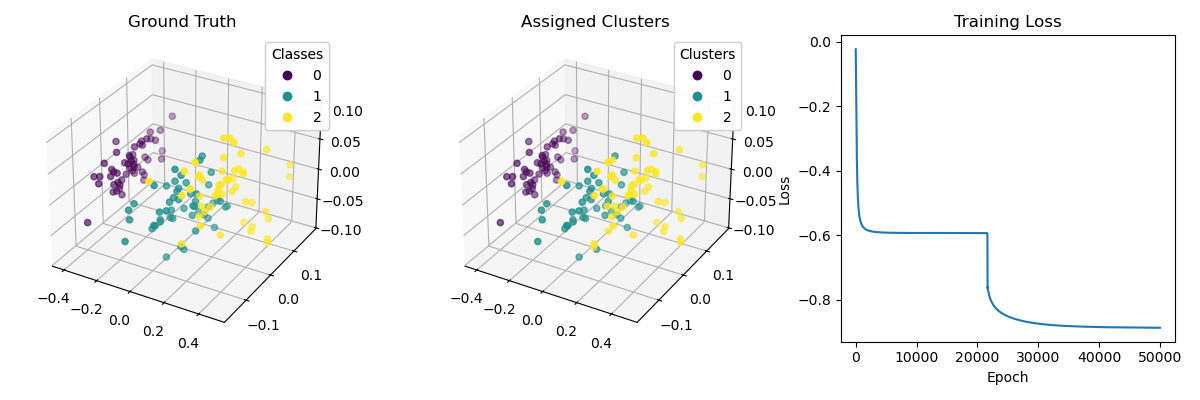
\includegraphics[width=1\linewidth]{Figure_1.png}%
    \caption{Comparison of ground truth (left), assigned clusters (middle), and training loss (right) using the Ising Clustering method.}
    \label{fig:comparison}
\end{figure*}

%\section{Results}
\section{Evaluation}

% We applied the analytical solution to the Iris dataset and compared it with classical clustering algorithms.

% \subsection{Implementation on Iris Dataset}

We employ a neural-network-based clustering model equipped with a softmax output layer. The model’s objective function is designed to maximize the pairwise differences in cluster assignments, encouraging data points to be placed into distinct clusters without relying on any explicit prior labels.

\subsection{Implementation}


To highlight the core principle of Ising Clustering, promoting well-separated cluster assignments purely through pairwise difference voting, we first test it on the Iris dataset~\cite{fisher1936use} using a simplified weighting scheme. Specifically, we set \( w_{ij} = 1 \) for all pairs \((i, j)\) to ensure that all pairwise relationships are treated equally. Under this uniform weighting, the algorithm achieves an Adjusted Rand Index (ARI) score of 0.9222, reflecting a high degree of agreement with the true class labels. Notably, this result is competitive with classical clustering methods, outperforming both K-Means~\cite{lloyd1982least} and Mean Shift~\cite{derpanis2005mean}, and closely approaching the performance of Agglomerative Clustering~\cite{murtagh2014ward}.

Beyond Iris, we also assess Ising Clustering on more complex datasets, reverting to the standard definition \( w_{ij} = \| \mathbf{x}_i - \mathbf{x}_j \|^2 \) to incorporate the intrinsic geometry of the data. As shown in Table~\ref{tab:results}, our method consistently exhibits strong clustering performance across a range of benchmark datasets, including Iris, Parkinsons~\cite{parkinsons_174}, Wisconsin (1992)~\cite{breast_cancer_wisconsin_(original)_15} and Wisconsin (1995)~\cite{breast_cancer_wisconsin_(diagnostic)_17}. While the classical algorithms sometimes outperforms Ising Clustering on certain datasets (such as K-Means on the Breast Cancer dataset), our approach generally remains competitive. In particular, on the Wisconsin (1992) dataset, Ising Clustering delivers the highest ARI score compared to the tested baseline methods, and on other datasets such as Wisconsin (1995), it similarly demonstrates strong performance.





\subsection{Results Visualization}

Figure~\ref{fig:comparison} provides a visual illustration of the clustering process and outcomes under the Ising Clustering framework. The left panel shows the ground truth distribution of the data samples, the middle panel presents the clusters assigned by our model, and the right panel displays the training loss curve throughout the optimization procedure. 

By comparing the ground truth classes and the assigned clusters, it becomes apparent that our method can distinguish between different classes without prior labeling. The training loss curve indicates that the model steadily converges towards a stable solution, further validating the effectiveness of the Ising Clustering approach.


\subsection{Adjusted Rand Index (ARI)}

We evaluated the clustering performance using the Adjusted Rand Index (ARI). The results are presented in Table~\ref{tab:results}.



\begin{table}[h!]
\centering
\caption{ARI Scores for Ising Clustering and Classical Algorithms}
\label{tab:results}
\begin{tabular}{@{}lcccc@{}}
\toprule
\textbf{Dataset} & \textbf{Ising} & \textbf{K-Means} & \textbf{Agglomerative} & \textbf{Mean Shift} \\ \midrule
% Iris & \textbf{0.6318} & 0.4328 & 0.6153 & 0.5681 \\
Iris & \textbf{0.9222} & 0.7163 & 0.7312 & 0.5584 \\
% Wine & \textbf{0.8516} & 0.8975 & 0.7899 & -0.0064 \\
% Breast Cancer & 0.6720 & \textbf{0.6765} & 0.5750 & 0.1279 \\
% Heart Disease & \textbf{0.3707} & 0.4293 & 0.1461 & 0.0000 \\
Parkinsons & \textbf{0.1275} & -0.0978 & 0.1267 & -0.1012 \\
% Diabetes & \textbf{0.0033} & 0.0997 & 0.1022 & 0.0262 \\
% Hepatitis & \textbf{0.2555} & 0.2521 & 0.3166 & -0.0106 \\
% Lymphography & \textbf{0.1522} & 0.0392 & 0.1747 & 0.0934 \\
Wisconsin (1992) & \textbf{0.8661} & 0.8126 & 0.8609 & 0.7175 \\
Wisconsin (1995) & \textbf{0.6604} & 0.6536 & 0.5750 & 0.1279 \\ \bottomrule
\end{tabular}
\end{table}





\subsection{Discussion}

% The Ising Clustering algorithm achieved an ARI score of 0.9222 on the Iris dataset using the analytical solution with softmax approximation. While this is better than other methods without dimension reduction, it demonstrates the potential of the method without complicated preprocessing.


The Ising Clustering algorithm achieves an ARI score of 0.9222 on the Iris dataset, outperforming classical algorithms such as K-Means (0.7163), Agglomerative Clustering (0.7312), and Mean Shift (0.5584). This demonstrates the effectiveness of our gradient-based optimization approach, which relies on the pairwise difference loss to discover well-separated clusters directly from the data without requiring complex preprocessing steps or prior assumptions about the data distribution.

On other datasets, the performance of Ising Clustering is competitive as well. For example, on the Wisconsin (1992) dataset, Ising Clustering achieves the highest ARI score of 0.8661, surpassing both K-Means (0.8126) and Mean Shift (0.7175) while slightly outperforming Agglomerative Clustering (0.8609). Similarly, on the Wisconsin (1995) dataset, the algorithm delivers the highest ARI score of 0.6604, slightly better than K-Means (0.6536) and significantly better than Mean Shift (0.1279).

These results highlight the versatility of Ising Clustering across datasets with varying structures and complexities. Notably, even without explicit dimensionality reduction or kernel transformations, the algorithm is capable of achieving strong performance by leveraging its inherent capacity to maximize pairwise differences in cluster probabilities. This positions Ising Clustering as a robust and flexible tool for unsupervised learning tasks, capable of handling both simple and complex datasets effectively.

% The competitive performance of the algorithm further underscores its potential as a principled alternative to classical clustering methods. Unlike K-Means or Agglomerative Clustering, which rely on explicit distance metrics or hierarchical merging, Ising Clustering operates through an optimization-driven framework that inherently adapts to the data distribution. This adaptability, coupled with the physical interpretability of its loss function, provides a promising foundation for extending the method to more challenging and high-dimensional datasets in the future.


\section{Conclusion}

In this paper, we introduce Ising Clustering, a novel algorithm inspired by the Ising model and democratic voting principles. We first formulate the clustering problem as a constrained optimization problem minimizing the weighted pairwise differences, and subsequently reformulate it into an unconstrained QUBO problem.  By employing a neural network and approximating the softmax function, we derive the final analytical solution for clustering tasks. In order to evaluate our proposed model, we conduct Ising Clustering experiments on different datasets, compared to conventional methods including K-Means, Agglomerative, and Mean Shift. The results indicate that our Ising model can outperform over most datasets, with steady performance and convergence rate.

Our approach provides insights into how clustering algorithms can be formulated using physical models, approximations and optimization tools, offering a foundation for further research into efficient clustering methods. We plan to further apply our method on neuromorphic imaging data for the identification of objects and moving tracks in the future. 

% \section{Future Work}

% \section*{Acknowledgments}

% We thank the research community for their valuable datasets and the open-source contributors for their tools.

\appendices



% \section*{References}
\bibliographystyle{IEEEtran}
\bibliography{ref}

\end{document}
